\newcommand{\titulus}{\nomenFesti{S. Callisti I, Papæ \& Martyris.}
\dies{Die 14. Octobris.}}
\newcommand{\sineobmv}{Sine officium B.M.V.}
\newcommand{\oratio}{\pars{Oratio.}

\noindent Preces pópuli tui, quǽsumus, Dómine, cleménter exáudi, ut beáti Callísti, papæ, méritis adiuvémur, cuius passióne lætámur.

\pars{Pro pace in universo mundo.} \scriptura{Sir. 50, 25; 2 Esdr. 4, 20; \textbf{H416}}

\vspace{-4mm}

\antiphona{II D}{temporalia/ant-dapacemdomine.gtex}

\vfill

\noindent Deus, a quo sancta desidéria, recta consília et iusta sunt ópera: da servis tuis illam, quam mundus dare non potest, pacem; ut et corda nostra mandátis tuis dédita, et hóstium subláta formídine, témpora sint tua protectióne tranquílla.

\noindent Per Dóminum nostrum Iesum Christum, Fílium tuum, qui tecum vivit et regnat in unitáte Spíritus Sancti, Deus, per ómnia sǽcula sæculórum.

\noindent \Rbardot{} Amen.}
\newcommand{\invitatorium}{\pars{Invitatorium.}

\vspace{-4mm}

\antiphona{E}{temporalia/inv-regemmartyrumsimplex.gtex}}
\newcommand{\hymnusmatutinum}{\pars{Hymnus}

\cuminitiali{I}{temporalia/hym-BeateMartyr.gtex}}
\newcommand{\matversus}{\noindent \Vbardot{} Fili mi, atténde ad sapiéntiam meam.

\noindent \Rbardot{} Et prudéntiæ meæ inclína aurem tuam.}
\newcommand{\lectioi}{\pars{Lectio I.} \scriptura{Ag. 2, 10-23}

\noindent De libro Aggǽi prophétæ.

\noindent In vicésima et quarta noni mensis, in anno secúndo Daríi, factum est verbum Dómini ad Aggǽum prophétam dicens: «Hæc dicit Dóminus exercítuum: Intérroga sacerdótes legem dicens: Si túlerit homo carnem sanctificátam in ora vestiménti sui et tetígerit de summitáte eius panem aut pulméntum aut vinum aut óleum aut omnem cibum, numquid sanctificábitur?». Respondéntes autem sacerdótes dixérunt: «Non». Et dixit Aggǽus: «Si tetígeris pollútus cadávere ómnia hæc, numquid contaminabúntur?». Et respondérunt sacerdótes et dixérunt: «Contaminabúntur». Et respóndit Aggǽus et dixit: «Sic pópulus iste et sic gens ista ante fáciem meam, dicit Dóminus, et sic omne opus mánuum eórum et ómnia, quæ ófferunt ibi, contamináta sunt.

\noindent Et nunc pónite corda vestra a die hac et supra: Antequam ponerétur lapis super lápidem in templo Dómini, quid fuístis? Cum accederétis ad acérvum vigínti modiórum, erant decem; cum intrarétis ad tórcular, ut haurirétis quinquagínta lagénas, erant vigínti. Percússi vos ariditáte et rubígine et grándine ómnia ópera mánuum vestrárum, et non fuit in vobis qui reverterétur ad me, dicit Dóminus. Pónite corda vestra ex die ista et in futúrum, a die vicésima et quarta noni mensis, a die, qua fundaménta iacta sunt templi Dómini, pónite super cor vestrum. Numquid adhuc semen in hórreo est, et adhuc vínea et ficus et malogranátum et lignum olívæ non portávit fructum? Ex die hac benedícam».

\noindent Et factum est verbum Dómini secúndo ad Aggǽum in vicésima et quarta mensis dicens: «Lóquere ad Zoróbabel ducem Iudæ dicens: Ego movébo cælum páriter et terram et subvértam sólium regnórum et cónteram fortitúdinem regnórum géntium et subvértam quadrígam et ascensóres eius; et descéndent equi et ascensóres eórum, unusquísque percússus gládio fratris sui. In die illo, dicit Dóminus exercítuum, assúmam te, Zoróbabel fili Saláthiel, serve meus, dicit Dóminus, et ponam te quasi signáculum, quia te elégi», dicit Dóminus exercítuum.}
\newcommand{\responsoriumi}{\pars{Responsorium 1.} \scriptura{\Rbar{} Cf. Is. 35, 2 \Vbar{} Is. 40, 10; \textbf{H35}}

\vspace{-5mm}

\responsorium{I}{temporalia/resp-germinaveruntcampi-CROCHU.gtex}{}

\vfill

\rubrica{vel ad libitum:}

\vspace{3mm}

\pars{Responsorium 1.} \scriptura{\Rbardot{} Ag. 2, 24 \Vbardot{} Ps. 80, 8; \textbf{H61}}

\vspace{-5mm}

\responsorium{VIII}{temporalia/resp-inillodiesuscipiam-CROCHU.gtex}{}}
\newcommand{\lectioii}{\pars{Lectio II.} \scriptura{Cap. 13: CSEL 3, 346-347}

\noindent Ex Tractátu sancti Cypriáni epíscopi et mártyris ad Fortunátum.

\noindent \emph{Non sunt condígnæ passiónes huius témporis ad superventúram claritúdinem quæ revelábitur in nobis.} Quis ergo non ómnibus modis elabóret ad claritátem tantam perveníre, ut amícus Dei fiat, ut cum Christo statim gáudeat, ut post torménta et supplícia terréna prǽmia divína percípiat? Si milítibus sæculáribus gloriósum est ut hoste devícto rédeant in pátriam triumphántes, quanto pótior et maior est glória victo diábolo ad paradísum triumphántem redíre et, unde Adam peccátor eiéctus est, illuc prostráto eo qui ante decéperat tropǽa victrícia reportáre, offérre Dómino acceptíssimum munus incorrúptam fidem, virtútem mentis incólumem, laudem devotiónis illústrem, comitári eum cum veníre cœ́perit vindíctam de inimícis receptúrus, láteri eius assístere cum séderit iudicatúrus, coherédem Christi fíeri, ángelis coæquári, cum patriárchis, cum apóstolis, cum prophétis cæléstis regni possessióne lætári.}
\newcommand{\responsoriumii}{\pars{Responsorium 2.} \scriptura{\textbf{H373}}

\vspace{-5mm}

\responsorium{III}{temporalia/resp-istecognovit-CROCHU.gtex}{}

\vfill
\pagebreak

\rubrica{vel ad libitum:}

\vspace{3mm}

\pars{Responsorium 2.}

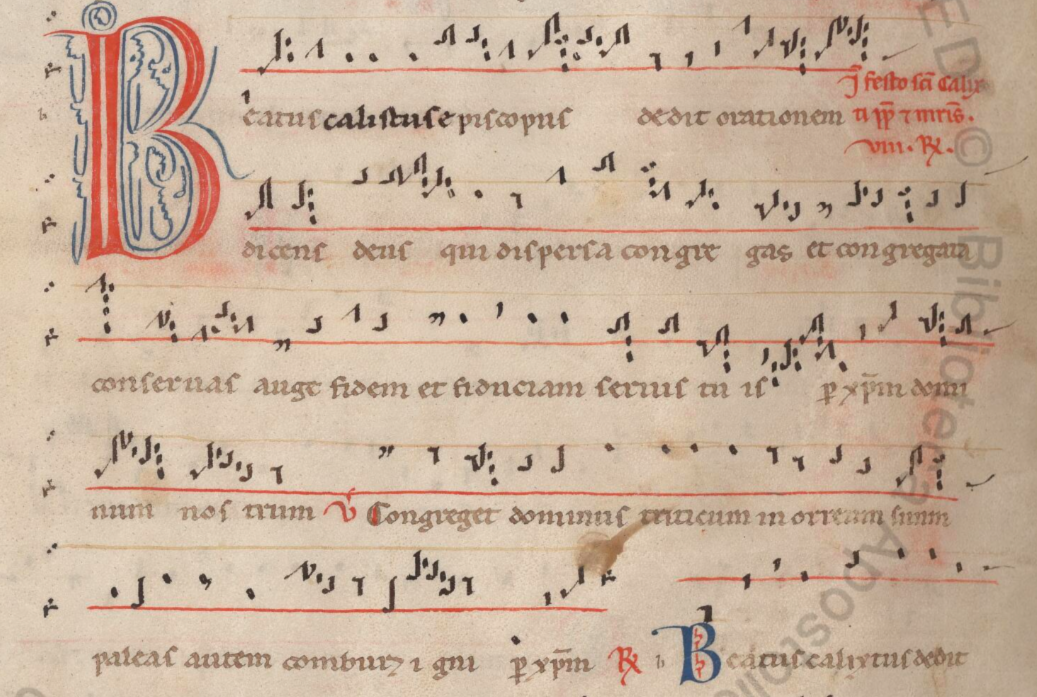
\includegraphics[width=17cm]{pic-beatuscallistus.png}}
\newcommand{\lectioiii}{\pars{Lectio III.}

\noindent Has cogitatiónes quæ persecútio potest víncere, quæ possunt torménta superáre? Durat fortis et stábilis religiósis meditatiónibus fundáta mens et advérsus omnes diáboli terróres et minas mundi ánimus immóbilis perstat, quem futurórum fides certa et sólida corróborat. Claudúntur in persecutiónibus terræ, sed patet cælum; minátur antichrístus, sed Christus tuétur; mors infértur, sed immortálitas séquitur. Quanta est dígnitas et quanta secúritas exíre hinc lætum, exíre inter pressúras et angústias gloriósum, cláudere in moménto óculos, quibus hómines videbántur et mundus, aperíre eósdem statim, ut Deus videátur et Christus. Tam felíciter migrándi quanta velócitas. Terris repénte subtráheris, ut in regnis cæléstibus reponáris.

\noindent Hæc opórtet mente et cogitatióne complécti, hæc die ac nocte meditári. Si talem persecútio invénerit Dei mílitem, vinci non póterit virtus ad prœ́lium prompta. Vel si arcessítio ante prævénerit, sine prǽmio non erit fides quæ erat ad martýrium præparáta; sine damno témporis merces Deo iúdice rédditur; in persecutióne milítia, in pace consciéntia coronátur.}
\newcommand{\responsoriumiii}{\pars{Responsorium 3.} \scriptura{\Rbardot{} Ps. 8, 6-8 \Vbardot{} Ps. 20, 4; \textbf{H374}}

\vspace{-5mm}

\responsorium{VII}{temporalia/resp-gloriaethonore-CROCHU-cumdox.gtex}{}}
\newcommand{\hymnuslaudes}{\pars{Hymnus}

\cuminitiali{VI}{temporalia/hym-MartyrDei.gtex}}
\newcommand{\lectiobrevis}{\pars{Lectio Brevis.} \scriptura{2 Cor. 1, 3-5}

\noindent Benedíctus Deus et Pater Dómini nostri Iesu Christi, Pater misericordiárum et Deus totíus consolatiónis, qui consolátur nos in omni tribulatióne nostra, ut possímus et ipsi consolári eos, qui in omni pressúra sunt, per exhortatiónem, qua exhortámur et ipsi a Deo; quóniam, sicut abúndant passiónes Christi in nobis, ita per Christum abúndat et consolátio.}
\newcommand{\responsoriumbreve}{\pars{Responsorium breve.} \scriptura{Ex. 15, 2}

\cuminitiali{VI}{temporalia/resp-fortitudomeaetlausmea.gtex}}
\newcommand{\preces}{\noindent Fratres, Salvatórem nostrum, testem fidélem, per mártyres interféctos propter verbum Dei,~\gredagger{} celebrémus, clamántes:

\Rbardot{} Redemísti nos Deo in sánguine tuo.

\noindent Per mártyres tuos, qui líbere mortem in testimónium fídei sunt ampléxi,~\gredagger{} da nobis, Dómine, veram spíritus libertátem.

\Rbardot{} Redemísti nos Deo in sánguine tuo.

\noindent Per mártyres tuos, qui fidem usque ad sánguinem sunt conféssi,~\gredagger{} da nobis, Dómine, puritátem fideíque constántiam.

\Rbardot{} Redemísti nos Deo in sánguine tuo.

\noindent Per mártyres tuos, qui, sustinéntes crucem, tua vestígia sunt secúti,~\gredagger{} da nobis, Dómine, ærúmnas vitæ fórtiter sustinére.

\Rbardot{} Redemísti nos Deo in sánguine tuo.

\noindent Per mártyres tuos, qui stolas suas lavérunt in sánguine Agni,~\gredagger{} da nobis, Dómine, omnes insídias carnis mundíque devíncere.

\Rbardot{} Redemísti nos Deo in sánguine tuo.}
\newcommand{\benedictus}{\pars{Canticum Zachariæ.} \scriptura{Io. 12, 35; \textbf{H375}}

\vspace{-4mm}

\antiphona{III a}{temporalia/ant-quisequiturmenonambulat.gtex}

%\vspace{-2mm}

\scriptura{Lc. 1, 68-79}

\vspace{-2mm}

\cantusSineNeumas
\initiumpsalmi{temporalia/benedictus-initium-iii-a-auto.gtex}

%\vspace{-1.5mm}

\input{temporalia/benedictus-iii-a.tex} \Abardot{}}
\newcommand{\benedicamuslaudes}{\cuminitiali{}{temporalia/benedicamus-memoria-laudes.gtex}}
\newcommand{\hebdomada}{infra Hebdom. XXVIII per Annum.}
%\newcommand{\hiemalis}{Hiemalis}
\newcommand{\matud}{Matutinum Hebdomadae D}
\newcommand{\matubd}{Matutinum Hebdomadae B vel D}
\newcommand{\laudd}{Laudes Hebdomadae D}
\newcommand{\laudbd}{Laudes Hebdomadae B vel D}

% LuaLaTeX

\documentclass[a4paper, twoside, 12pt]{article}
\usepackage[latin]{babel}
%\usepackage[landscape, left=3cm, right=1.5cm, top=2cm, bottom=1cm]{geometry} % okraje stranky
%\usepackage[landscape, a4paper, mag=1166, truedimen, left=2cm, right=1.5cm, top=1.6cm, bottom=0.95cm]{geometry} % okraje stranky
\usepackage[landscape, a4paper, mag=1400, truedimen, left=0.5cm, right=0.5cm, top=0.5cm, bottom=0.5cm]{geometry} % okraje stranky

\usepackage{fontspec}
\setmainfont[FeatureFile={junicode.fea}, Ligatures={Common, TeX}, RawFeature=+fixi]{Junicode}
%\setmainfont{Junicode}

% shortcut for Junicode without ligatures (for the Czech texts)
\newfontfamily\nlfont[FeatureFile={junicode.fea}, Ligatures={Common, TeX}, RawFeature=+fixi]{Junicode}

\usepackage{multicol}
\usepackage{color}
\usepackage{lettrine}
\usepackage{fancyhdr}

% usual packages loading:
\usepackage{luatextra}
\usepackage{graphicx} % support the \includegraphics command and options
\usepackage{gregoriotex} % for gregorio score inclusion
\usepackage{gregoriosyms}
\usepackage{wrapfig} % figures wrapped by the text
\usepackage{parcolumns}
\usepackage[contents={},opacity=1,scale=1,color=black]{background}
\usepackage{tikzpagenodes}
\usepackage{calc}
\usepackage{longtable}
\usetikzlibrary{calc}

\setlength{\headheight}{14.5pt}

% Commands used to produce a typical "Conventus" booklet

\newenvironment{titulusOfficii}{\begin{center}}{\end{center}}
\newcommand{\dies}[1]{#1

}
\newcommand{\nomenFesti}[1]{\textbf{\Large #1}

}
\newcommand{\celebratio}[1]{#1

}

\newcommand{\hora}[1]{%
\vspace{0.5cm}{\large \textbf{#1}}

\fancyhead[LE]{\thepage\ / #1}
\fancyhead[RO]{#1 / \thepage}
\addcontentsline{toc}{subsection}{#1}
}

% larger unit than a hora
\newcommand{\divisio}[1]{%
\begin{center}
{\Large \textsc{#1}}
\end{center}
\fancyhead[CO,CE]{#1}
\addcontentsline{toc}{section}{#1}
}

% a part of a hora, larger than pars
\newcommand{\subhora}[1]{
\begin{center}
{\large \textit{#1}}
\end{center}
%\fancyhead[CO,CE]{#1}
\addcontentsline{toc}{subsubsection}{#1}
}

% rubricated inline text
\newcommand{\rubricatum}[1]{\textit{#1}}

% standalone rubric
\newcommand{\rubrica}[1]{\vspace{3mm}\rubricatum{#1}}

\newcommand{\notitia}[1]{\textcolor{red}{#1}}

\newcommand{\scriptura}[1]{\hfill \small\textit{#1}}

\newcommand{\translatioCantus}[1]{\vspace{1mm}%
{\noindent\footnotesize \nlfont{#1}}}

% pruznejsi varianta nasledujiciho - umoznuje nastavit sirku sloupce
% s prekladem
\newcommand{\psalmusEtTranslatioB}[3]{
  \vspace{0.5cm}
  \begin{parcolumns}[colwidths={2=#3}, nofirstindent=true]{2}
    \colchunk{
      \input{#1}
    }

    \colchunk{
      \vspace{-0.5cm}
      {\footnotesize \nlfont
        \input{#2}
      }
    }
  \end{parcolumns}
}

\newcommand{\psalmusEtTranslatio}[2]{
  \psalmusEtTranslatioB{#1}{#2}{8.5cm}
}


\newcommand{\canticumMagnificatEtTranslatio}[1]{
  \psalmusEtTranslatioB{#1}{temporalia/extra-adventum-vespers/magnificat-boh.tex}{12cm}
}
\newcommand{\canticumBenedictusEtTranslatio}[1]{
  \psalmusEtTranslatioB{#1}{temporalia/extra-adventum-laudes/benedictus-boh.tex}{10.5cm}
}

% volne misto nad antifonami, kam si zpevaci dokresli neumy
\newcommand{\hicSuntNeumae}{\vspace{0.5cm}}

% prepinani mista mezi notovymi osnovami: pro neumovane a neneumovane zpevy
\newcommand{\cantusCumNeumis}{
  \setgrefactor{17}
  \global\advance\grespaceabovelines by 5mm%
}
\newcommand{\cantusSineNeumas}{
  \setgrefactor{17}
  \global\advance\grespaceabovelines by -5mm%
}

% znaky k umisteni nad inicialu zpevu
\newcommand{\superInitialam}[1]{\gresetfirstlineaboveinitial{\small {\textbf{#1}}}{\small {\textbf{#1}}}}

% pars officii, i.e. "oratio", ...
\newcommand{\pars}[1]{\textbf{#1}}

\newenvironment{psalmus}{
  \setlength{\parindent}{0pt}
  \setlength{\parskip}{5pt}
}{
  \setlength{\parindent}{10pt}
  \setlength{\parskip}{10pt}
}

%%%% Prejmenovat na latinske:
\newcommand{\nadpisZalmu}[1]{
  \hspace{2cm}\textbf{#1}\vspace{2mm}%
  \nopagebreak%

}

% mode, score, translation
\newcommand{\antiphona}[3]{%
\hicSuntNeumae
\superInitialam{#1}
\includescore{#2}

#3
}
 % Often used macros

\newcommand{\annusEditionis}{2021}

%%%% Vicekrat opakovane kousky

\newcommand{\anteOrationem}{
  \rubrica{Ante Orationem, cantatur a Superiore:}

  \pars{Supplicatio Litaniæ.}

  \cuminitiali{}{temporalia/supplicatiolitaniae.gtex}

  \pars{Oratio Dominica.}

  \cuminitiali{}{temporalia/oratiodominica.gtex}

  \rubrica{Deinde dicitur ab Hebdomadario:}

  \cuminitiali{}{temporalia/dominusvobiscum-solemnis.gtex}

  \rubrica{In choro monialium loco Dominus vobiscum dicitur:}

  \sineinitiali{temporalia/domineexaudi.gtex}
}

\setlength{\columnsep}{30pt} % prostor mezi sloupci

%%%%%%%%%%%%%%%%%%%%%%%%%%%%%%%%%%%%%%%%%%%%%%%%%%%%%%%%%%%%%%%%%%%%%%%%%%%%%%%%%%%%%%%%%%%%%%%%%%%%%%%%%%%%%
\begin{document}

% Here we set the space around the initial.
% Please report to http://home.gna.org/gregorio/gregoriotex/details for more details and options
\grechangedim{afterinitialshift}{2.2mm}{scalable}
\grechangedim{beforeinitialshift}{2.2mm}{scalable}
\grechangedim{interwordspacetext}{0.22 cm plus 0.15 cm minus 0.05 cm}{scalable}%
\grechangedim{annotationraise}{-0.2cm}{scalable}

% Here we set the initial font. Change 38 if you want a bigger initial.
% Emit the initials in red.
\grechangestyle{initial}{\color{red}\fontsize{38}{38}\selectfont}

\pagestyle{empty}

%%%% Titulni stranka
\begin{titulusOfficii}
\ifx\titulus\undefined
\nomenFesti{Feria II \hebdomada{}}
\else
\titulus
\fi
\end{titulusOfficii}

\vfill

\begin{center}
%Ad usum et secundum consuetudines chori \guillemotright{}Conventus Choralis\guillemotleft.

%Editio Sancti Wolfgangi \annusEditionis
\end{center}

\scriptura{}

\pars{}

\pagebreak

\renewcommand{\headrulewidth}{0pt} % no horiz. rule at the header
\fancyhf{}
\pagestyle{fancy}

\cantusSineNeumas

\hora{Ad Matutinum.} %%%%%%%%%%%%%%%%%%%%%%%%%%%%%%%%%%%%%%%%%%%%%%%%%%%%%

\vspace{2mm}

\cuminitiali{}{temporalia/dominelabiamea.gtex}

\vfill
%\pagebreak

\vspace{2mm}

\ifx\invitatorium\undefined
\pars{Invitatorium.} \scriptura{Lc. 24, 34; Psalmus 94; \textbf{H232}}

\vspace{-6mm}

\antiphona{VI}{temporalia/inv-surrexitdominusvere.gtex}
\else
\invitatorium
\fi

\vfill
\pagebreak

\ifx\hymnusmatutinum\undefined
\pars{Hymnus}

\cuminitiali{VIII}{temporalia/hym-LaetareCaelum.gtex}
\else
\hymnusmatutinum
\fi

\vspace{-3mm}

\vfill
\pagebreak

\ifx\matua\undefined
\else
% MAT A
\pars{Psalmus 1.} \scriptura{Ps. 6, 3}

\vspace{-4mm}

\antiphona{IV E}{temporalia/ant-misereremihi.gtex}

%\vspace{-2mm}

\scriptura{Ps. 6}

%\vspace{-2mm}

\initiumpsalmi{temporalia/ps6-initium-iv-E-auto.gtex}

\input{temporalia/ps6-iv-E.tex} \Abardot{}

\vfill
\pagebreak

\pars{Psalmus 2.} \scriptura{Ps. 110, 1; \textbf{H91}}

\vspace{-4mm}

\antiphona{VIII G}{temporalia/ant-confitebortibi.gtex}

%\vspace{-2mm}

\scriptura{Ps. 9, 2-11}

%\vspace{-2mm}

\initiumpsalmi{temporalia/ps9ii_xi-initium-viii-G-auto.gtex}

\input{temporalia/ps9ii_xi-viii-G.tex} \Abardot{}

\vfill
\pagebreak

\pars{Psalmus 3.} \scriptura{Ps. 9, 20}

\vspace{-4mm}

\antiphona{I g\textsuperscript{3}}{temporalia/ant-exsurgedominenon.gtex}

%\vspace{-2mm}

\scriptura{Ps. 9, 12-21}

%\vspace{-2mm}

\initiumpsalmi{temporalia/ps9xii_xxi-initium-i-g3-auto.gtex}

\input{temporalia/ps9xii_xxi-i-g3.tex} \Abardot{}

\vfill
\pagebreak
\fi
\ifx\matub\undefined
\else
% MAT B
\pars{Psalmus 1.} \scriptura{Ps. 30, 2; \textbf{H90}}

\vspace{-4mm}

\antiphona{VIII G}{temporalia/ant-intuaiustitia.gtex}

%\vspace{-2mm}

\scriptura{Ps. 30, 2-9}

%\vspace{-2mm}

\initiumpsalmi{temporalia/ps30i-initium-viii-G-auto.gtex}

\vspace{-1.5mm}

\input{temporalia/ps30i-viii-G.tex} \Abardot{}

\vfill
\pagebreak

\pars{Psalmus 2.} \scriptura{Ps. 66, 2}

\vspace{-4mm}

\antiphona{E}{temporalia/ant-illuminadomine.gtex}

%\vspace{-2mm}

\scriptura{Ps. 30, 10-17}

%\vspace{-2mm}

\initiumpsalmi{temporalia/ps30ii-initium-e-a-auto.gtex}

\input{temporalia/ps30ii-e-a.tex} \Abardot{}

\vfill
\pagebreak

\pars{Psalmus 3.} \scriptura{Ps. 30, 24}

\vspace{-4mm}

\antiphona{II D}{temporalia/ant-diligitedominum.gtex}

%\vspace{-5mm}

\scriptura{Ps. 30, 20-25}

%\vspace{-2mm}

\initiumpsalmi{temporalia/ps30iii-initium-ii-D-auto.gtex}

\input{temporalia/ps30iii-ii-D.tex} \Abardot{}

\vfill
\pagebreak
\fi
\ifx\matuc\undefined
\else
% MAT C
\pars{Psalmus 1.}

\vspace{-4mm}

\antiphona{VIII G\textsuperscript{3}}{temporalia/ant-alleluia-bv21-n4.gtex}

%\vspace{-2mm}

\scriptura{Ps. 49, 1-6}

%\vspace{-2mm}

\initiumpsalmi{temporalia/ps49i_vi-initium-viii-G3.gtex}

\input{temporalia/ps49i_vi-viii-G2.tex}

\vfill
\pagebreak

\pars{Psalmus 2.}

\scriptura{Ps. 49, 7-15}

%\vspace{-2mm}

\initiumpsalmi{temporalia/ps49vii_xv-initium-viii-G3.gtex}

\input{temporalia/ps49vii_xv-viii-G2.tex}

\vfill
\pagebreak

\pars{Psalmus 3.}

\scriptura{Ps. 49, 16-23}

%\vspace{-2mm}

\initiumpsalmi{temporalia/ps49xvi_xxiii-initium-viii-G3.gtex}

\input{temporalia/ps49xvi_xxiii-viii-G2.tex} \Abardot{}

\vfill
\pagebreak
\fi
\ifx\matud\undefined
\else
% MAT D
\pars{Psalmus 1.} \scriptura{Ps. 72, 1}

\vspace{-4mm}

\antiphona{VIII c}{temporalia/ant-quambonusdeus.gtex}

%\vspace{-2mm}

\scriptura{Ps. 72, 1-12}

%\vspace{-2mm}

\initiumpsalmi{temporalia/ps72i-initium-viii-c-auto.gtex}

%\vspace{-1.5mm}

\input{temporalia/ps72i-viii-c.tex} \Abardot{}

\vfill
\pagebreak

\pars{Psalmus 2.} \scriptura{Ps. 15, 7; \textbf{H99}}

\vspace{-4mm}

\antiphona{II D}{temporalia/ant-benedicamdomino.gtex}

%\vspace{-2mm}

\scriptura{Ps. 72, 13-20}

%\vspace{-2mm}

\initiumpsalmi{temporalia/ps72ii-initium-ii-D-auto.gtex}

\input{temporalia/ps72ii-ii-D.tex} \Abardot{}

\vfill
\pagebreak

\pars{Psalmus 3.} \scriptura{Ps. 72, 28}

\vspace{-4mm}

\antiphona{III b}{temporalia/ant-adhaereredeobonumest.gtex}

%\vspace{-2mm}

\scriptura{Ps. 72, 21-28}

%\vspace{-2mm}

\initiumpsalmi{temporalia/ps72iii-initium-iii-b.gtex}

\input{temporalia/ps72iii-iii-b.tex} \Abardot{}

\vfill
\pagebreak
\fi

\pars{Versus.}

\ifx\matversus\undefined
\ifx\matua\undefined
\else
\noindent \Vbardot{} Da mihi intelléctum et servábo legem tuam. 

\noindent \Rbardot{} Et custódiam illam in toto corde meo.
\fi
\ifx\matub\undefined
\else
\noindent \Vbardot{} Dírige me, Dómine, in veritáte tua, et doce me.

\noindent \Rbardot{} Quia tu es Deus salútis meæ.
\fi
\ifx\matuc\undefined
\else
\noindent \Vbardot{} Cor meum et caro mea, allelúia.

\noindent \Rbardot{} Exsultavérunt in Deum vivum, allelúia.
\fi
\ifx\matud\undefined
\else
\noindent \Vbardot{} Quam dúlcia fáucibus meis elóquia tua, Dómine.

\noindent \Rbardot{} Super mel ori meo.
\fi
\else
\matversus
\fi

\vspace{5mm}

\sineinitiali{temporalia/oratiodominica-mat.gtex}

\vspace{5mm}

\pars{Absolutio.}

\cuminitiali{}{temporalia/absolutio-exaudi.gtex}

\vfill
\pagebreak

\cuminitiali{}{temporalia/benedictio-solemn-benedictione.gtex}

\vspace{7mm}

\lectioi

\noindent \Vbardot{} Tu autem, Dómine, miserére nobis.
\noindent \Rbardot{} Deo grátias.

\vfill
\pagebreak

\responsoriumi

\vfill
\pagebreak

\cuminitiali{}{temporalia/benedictio-solemn-unigenitus.gtex}

\vspace{7mm}

\lectioii

\noindent \Vbardot{} Tu autem, Dómine, miserére nobis.
\noindent \Rbardot{} Deo grátias.

\vfill
\pagebreak

\responsoriumii

\vfill
\pagebreak

\cuminitiali{}{temporalia/benedictio-solemn-spiritus.gtex}

\vspace{7mm}

\lectioiii

\noindent \Vbardot{} Tu autem, Dómine, miserére nobis.
\noindent \Rbardot{} Deo grátias.

\vfill
\pagebreak

\responsoriumiii

\vfill
\pagebreak

\rubrica{Reliqua omittuntur, nisi Laudes separandæ sint.}

\sineinitiali{temporalia/domineexaudi.gtex}

\vfill

\oratio

\vfill

\noindent \Vbardot{} Dómine, exáudi oratiónem meam.
\Rbardot{} Et clamor meus ad te véniat.

\vfill

\noindent \Vbardot{} Benedicámus Dómino.
\noindent \Rbardot{} Deo grátias.

\vfill

\noindent \Vbardot{} Fidélium ánimæ per misericórdiam Dei requiéscant in pace.
\Rbardot{} Amen.

\vfill
\pagebreak

\hora{Ad Laudes.} %%%%%%%%%%%%%%%%%%%%%%%%%%%%%%%%%%%%%%%%%%%%%%%%%%%%%

\cantusSineNeumas

\vspace{0.5cm}
\grechangedim{interwordspacetext}{0.18 cm plus 0.15 cm minus 0.05 cm}{scalable}%
\cuminitiali{}{temporalia/deusinadiutorium-communis.gtex}
\grechangedim{interwordspacetext}{0.22 cm plus 0.15 cm minus 0.05 cm}{scalable}%

\vfill
\pagebreak

\ifx\hymnuslaudes\undefined
\ifx\laudac\undefined
\else
\pars{Hymnus}

\cuminitiali{I}{temporalia/hym-ChorusNovae-praglia.gtex}
\fi
\ifx\laudbd\undefined
\else
\pars{Hymnus}

\cuminitiali{I}{temporalia/hym-ChorusNovae.gtex}
\vspace{-3mm}
\fi
\else
\hymnuslaudes
\fi

\vfill
\pagebreak

\ifx\lauda\undefined
\else
\pars{Psalmus 1.} \scriptura{Ps. 5, 2; \textbf{H93}}

\vspace{-6mm}

\antiphona{VIII a}{temporalia/ant-intellegeclamorem.gtex}

\vspace{-4mm}

\scriptura{Psalmus 5.}

\vspace{-2mm}

\initiumpsalmi{temporalia/ps5-initium-viii-A-auto.gtex}

\vspace{-1.5mm}

\input{temporalia/ps5-viii-A.tex} \Abardot{}

\vfill
\pagebreak

\pars{Psalmus 2.} \scriptura{1 Par. 29, 13}

\vspace{-4mm}

\antiphona{I f}{temporalia/ant-laudamusnomentuum.gtex}

%\vspace{-2mm}

\scriptura{Canticum David, 1 Par. 29, 10-13}

%\vspace{-2mm}

\initiumpsalmi{temporalia/david-initium-i-f-auto.gtex}

\input{temporalia/david-i-f.tex} \Abardot{}

\vfill
\pagebreak

\pars{Psalmus 3.} \scriptura{Ps. 28, 1.2; \textbf{H72}}

\vspace{-4mm}

\antiphona{VII a}{temporalia/ant-affertedomino.gtex}

\scriptura{Psalmus. 28}

\initiumpsalmi{temporalia/ps28-initium-vii-a-auto.gtex}

\input{temporalia/ps28-vii-a.tex} \Abardot{}

\vfill
\pagebreak
\fi
\ifx\laudb\undefined
\else
\pars{Psalmus 1.} \scriptura{Ps. 41, 3; \textbf{H391}}

\vspace{-4mm}

\antiphona{II D}{temporalia/ant-sitivitanima.gtex}

%\vspace{-2mm}

\scriptura{Psalmus 41}

%\vspace{-2mm}

\initiumpsalmi{temporalia/ps41-initium-ii-D-auto.gtex}

%\vspace{-1.5mm}

\input{temporalia/ps41-ii-D.tex}

\vfill

\antiphona{}{temporalia/ant-sitivitanima.gtex}

\vfill
\pagebreak

\pars{Psalmus 2.}

\vspace{-4mm}

\antiphona{III a}{temporalia/ant-ostendenobisdomine.gtex}

%\vspace{-2mm}

\scriptura{Canticum Ecclesiastici, Sir. 36, 1-7.13-16}

%\vspace{-3mm}

\initiumpsalmi{temporalia/ecclesiastici-initium-iii-a-auto.gtex}

\input{temporalia/ecclesiastici-iii-a.tex} \Abardot{}

\vfill
\pagebreak

\pars{Psalmus 3.}

\vspace{-4mm}

\antiphona{II D}{temporalia/ant-operamanuumeius.gtex}

\scriptura{Psalmus 18, 1-7}

\initiumpsalmi{temporalia/ps18i-initium-ii-D-auto.gtex}

\input{temporalia/ps18i-ii-D.tex} \Abardot{}

\vfill
\pagebreak
\fi
\ifx\laudc\undefined
\else
\pars{Psalmus 1.}

\vspace{-4mm}

\antiphona{VIII G}{temporalia/ant-alleluia-turco12.gtex}

%\vspace{-2mm}

\scriptura{Psalmus 83}

%\vspace{-2mm}

\initiumpsalmi{temporalia/ps83-initium-viii-G-auto.gtex}

%\vspace{-1.5mm}

\input{temporalia/ps83-viii-G.tex} \Abardot{}

\vfill
\pagebreak

\pars{Psalmus 2.} \scriptura{Mi. 4, 2}

\vspace{-4mm}

\antiphona{VIII G\textsuperscript{2}}{temporalia/ant-veniteascendamus-tp.gtex}

%\vspace{-2mm}

\scriptura{Canticum Isaiæ, Is. 2, 2-5}

%\vspace{-2mm}

\initiumpsalmi{temporalia/isaiae11-initium-viii-g5-auto.gtex}

\input{temporalia/isaiae11-viii-g5.tex} \Abardot{}

\vfill
\pagebreak

\pars{Psalmus 3.}

\vspace{-4mm}

\antiphona{II D}{temporalia/ant-alleluia-turco8.gtex}

\scriptura{Psalmus 95}

\initiumpsalmi{temporalia/ps95-initium-ii-D-auto.gtex}

\input{temporalia/ps95-ii-D.tex} \Abardot{}

\vfill
\pagebreak
\fi
\ifx\laudd\undefined
\else
\pars{Psalmus 1.} \scriptura{Ps. 89, 1; \textbf{H98}}

\vspace{-4mm}

\antiphona{VI F}{temporalia/ant-dominerefugium.gtex}

%\vspace{-2mm}

\scriptura{Psalmus 89}

%\vspace{-2mm}

\initiumpsalmi{temporalia/ps89-initium-vi-F-auto.gtex}

%\vspace{-1.5mm}

\input{temporalia/ps89-vi-F.tex}

\vfill

\antiphona{}{temporalia/ant-dominerefugium.gtex}

\vfill
\pagebreak

\pars{Psalmus 2.} \scriptura{Is. 42, 10; \textbf{H98}}

\vspace{-4mm}

\antiphona{VI F}{temporalia/ant-cantatedominocanticum.gtex}

%\vspace{-2mm}

\scriptura{Canticum Isaiæ, Is. 42, 10-16}

%\vspace{-3mm}

\initiumpsalmi{temporalia/isaiae10-initium-vi-F-auto.gtex}

\input{temporalia/isaiae10-vi-F.tex} \Abardot{}

\vfill
\pagebreak

\pars{Psalmus 3.} \scriptura{Ps. 134, 1-2}

\vspace{-4mm}

\antiphona{I a}{temporalia/ant-laudatenomendomini.gtex}

\scriptura{Psalmus 134, 1-12}

\initiumpsalmi{temporalia/ps134i-initium-i-a-auto.gtex}

\input{temporalia/ps134i-i-a.tex} \Abardot{}

\vfill
\pagebreak
\fi

\ifx\lectiobrevis\undefined
\ifx\lauda\undefined
\else
\pars{Lectio Brevis.} \scriptura{2 Th. 3, 10-13}

\noindent Si quis non vult operári, nec mandúcet. Audímus enim inter vos quosdam ambuláre inordináte, nihil operántes sed curióse agéntes; his autem, qui eiúsmodi sunt, præcípimus et obsecrámus in Dómino Iesu Christo, ut cum quiéte operántes suum panem mandúcent. Vos autem, fratres, nolíte defícere benefaciéntes.
\fi
\ifx\laudb\undefined
\else
\pars{Lectio Brevis.} \scriptura{Ier. 15, 16}

\noindent Invénti sunt sermónes tui, et comédi eos, et factum est mihi verbum tuum in gáudium et in lætítiam cordis mei, quóniam invocátum est nomen tuum super me, Dómine Deus exercítuum.
\fi
\ifx\laudc\undefined
\else
\pars{Lectio Brevis.} \scriptura{Rom. 10, 8-10}

\noindent Prope te est verbum, in ore tuo et in corde tuo; hoc est verbum fídei, quod prædicámus. Quia si confiteáris in ore tuo: «Dóminum Iesum!», et in corde tuo credíderis quod Deus illum excitávit ex mórtuis, salvus eris. Corde enim créditur ad iustítiam, ore autem conféssio fit in salútem.
\fi
\ifx\laudd\undefined
\else
\pars{Lectio Brevis.} \scriptura{Idt. 8, 25-27}

\noindent Grátias agámus Dómino Deo nostro, qui temptat nos sicut et patres nostros. Mémores estóte quanta fécerit cum Abraham et Isaac, et quanta facta sint Iacob. Quia non sicut illos combússit in inquisitiónem cordis illórum et in nos non ultus est, sed in monitiónem flagéllat Dóminus appropinquántes sibi.
\fi
\else
\lectiobrevis
\fi

\vfill

\ifx\responsoriumbreve\undefined
\pars{Responsorium breve.} \scriptura{Cf. Mt. 28, 6; Cf. Gal. 3, 13}

\cuminitiali{VI}{temporalia/resp-surrexitdominusdesepulcro.gtex}
\else
\responsoriumbreve
\fi

\vfill
\pagebreak

\benedictus

\vspace{-1cm}

\vfill
\pagebreak

\pars{Preces.}

\sineinitiali{}{temporalia/tonusprecum.gtex}

\ifx\preces\undefined
\ifx\lauda\undefined
\else
\noindent Christum magnificémus, plenum grátia et Spíritu Sancto, \gredagger{} et fidénter eum implorémus:

\Rbardot{} Spíritum tuum da nobis, Dómine.

\noindent Concéde nobis diem istum iucúndum, pacíficum et sine mácula, \gredagger{} ut, ad vésperam perdúcti, cum gáudio et mundo corde te collaudáre valeámus.

\Rbardot{} Spíritum tuum da nobis, Dómine.

\noindent Sit hódie splendor tuus super nos, \gredagger{} et opus mánuum nostrárum dírige.

\Rbardot{} Spíritum tuum da nobis, Dómine.

\noindent Osténde fáciem tuam super nos ad bonum in pace, \gredagger{} ut hódie manu tua válida contegámur.

\Rbardot{} Spíritum tuum da nobis, Dómine.

\noindent Réspice propítius omnes, qui oratiónibus nostris confídunt, \gredagger{} eos adímple bonis ánimæ et córporis univérsis.

\Rbardot{} Spíritum tuum da nobis, Dómine.
\fi
\ifx\laudb\undefined
\else
\noindent Salvátor noster fecit nos regnum et sacerdótium, ut hóstias Deo acceptábiles offerámus. \gredagger{} Grati ígitur eum invocémus:

\Rbardot{} Serva nos in tuo ministério, Dómine.

\noindent Christe, sacérdos ætérne, qui sanctum pópulo tuo sacerdótium concessísti, \gredagger{} concéde, ut spiritáles hóstias Deo acceptábiles iúgiter offerámus.

\Rbardot{} Serva nos in tuo ministério, Dómine.

\noindent Spíritus tui fructus nobis largíre propítius, \gredagger{} patiéntiam, benignitátem et mansuetúdinem.

\Rbardot{} Serva nos in tuo ministério, Dómine.

\noindent Da nobis te amáre, ut te, qui es cáritas, possideámus, \gredagger{} et bene ágere, ut per vitam étiam nostram te laudémus.

\Rbardot{} Serva nos in tuo ministério, Dómine.

\noindent Quæ frátribus nostris sunt utília, nos quǽrere concéde, \gredagger{} ut salútem facílius consequántur.

\Rbardot{} Serva nos in tuo ministério, Dómine.
\fi
\ifx\laudc\undefined
\else
\noindent Iesum, quem Pater glorificávit et herédem ómnium géntium constítuit, \gredagger{} exaltémus, orántes:

\Rbardot{} Per victóriam tuam salva nos, Dómine.

\noindent Christe, qui victória tua portas contrivísti infernáles, peccátum delens et mortem, \gredagger{} fac nos hódie peccáti victóres.

\Rbardot{} Per victóriam tuam salva nos, Dómine.

\noindent Tu, qui mortem evacuásti, vitam nobis impértiens novam, \gredagger{} da ut hódie in hac vitæ novitáte ambulémus.

\Rbardot{} Per victóriam tuam salva nos, Dómine.

\noindent Qui vitam mórtuis tribuísti, totum genus humánum de morte ad vitam redúcens, \gredagger{} ómnibus, qui nobis occúrrent, ætérnam vitam concéde.

\Rbardot{} Per victóriam tuam salva nos, Dómine.

\noindent Qui, sepúlcri tui custódes confúndens, discípulos tuos lætificásti, \gredagger{} plenam tibi serviéntibus largíre lætítiam.

\Rbardot{} Per victóriam tuam salva nos, Dómine.
\fi
\ifx\laudd\undefined
\else
\noindent Christum, qui exáudit et salvos facit sperántes in se, \gredagger{} precémur acclamántes:

\Rbardot{} Te laudámus, in te sperámus, Dómine.

\noindent Grátias ágimus tibi, qui dives es in misericórdia, \gredagger{} propter nímiam caritátem, qua dilexísti nos.

\Rbardot{} Te laudámus, in te sperámus, Dómine.

\noindent Qui omni témpore in mundo cum Patre operáris, \gredagger{} nova fac ómnia per Spíritus Sancti virtútem.

\Rbardot{} Te laudámus, in te sperámus, Dómine.

\noindent Aperi óculos nostros et fratrum nostrórum, \gredagger{} ut videámus hódie mirabília tua.

\Rbardot{} Te laudámus, in te sperámus, Dómine.

\noindent Qui nos hódie ad tuum servítium vocas, \gredagger{} nos erga fratres multifórmis grátiæ tuæ fac minístros.

\Rbardot{} Te laudámus, in te sperámus, Dómine.
\fi
\else
\preces
\fi

\vfill

\pars{Oratio Dominica.}

\cuminitiali{}{temporalia/oratiodominicaalt.gtex}

\vfill
\pagebreak

\rubrica{vel:}

\pars{Supplicatio Litaniæ.}

\cuminitiali{}{temporalia/supplicatiolitaniae.gtex}

\vfill

\pars{Oratio Dominica.}

\cuminitiali{}{temporalia/oratiodominica.gtex}

\vfill
\pagebreak

% Oratio. %%%
\oratio

\vspace{-1mm}

\vfill

\rubrica{Hebdomadarius dicit Dominus vobiscum, vel, absente sacerdote vel diacono, sic concluditur:}

\vspace{2mm}

\antiphona{C}{temporalia/dominusnosbenedicat.gtex}

\rubrica{Postea cantatur a cantore:}

\vspace{2mm}

\cuminitiali{VII}{temporalia/benedicamus-tempore-paschali.gtex}

\vspace{1mm}

\vfill
\pagebreak

\end{document}

